\section{Binary Outcome Models}

    \subsection{Naïve Logit and Probit}
        Naïve estimations of 
        \begin{align}
            \mathbb{P}(\texttt{Vote} = 1 \vert x) = \Lambda(x'\beta) 
            \label{eq_bin_logit}
            \\
            \mathbb{P}(\texttt{Vote} = 1 \vert x) = \Phi(x'\beta) 
            \label{eq_bin_probit}
        \end{align}
        using logit (regression \ref{eq_bin_logit}) and probit (regression \ref{eq_bin_probit}) are presented in Figures \ref{fig_11_log} and \ref{fig_11_prob}, respectively.
            \begin{figure}[!htb]
                \centering 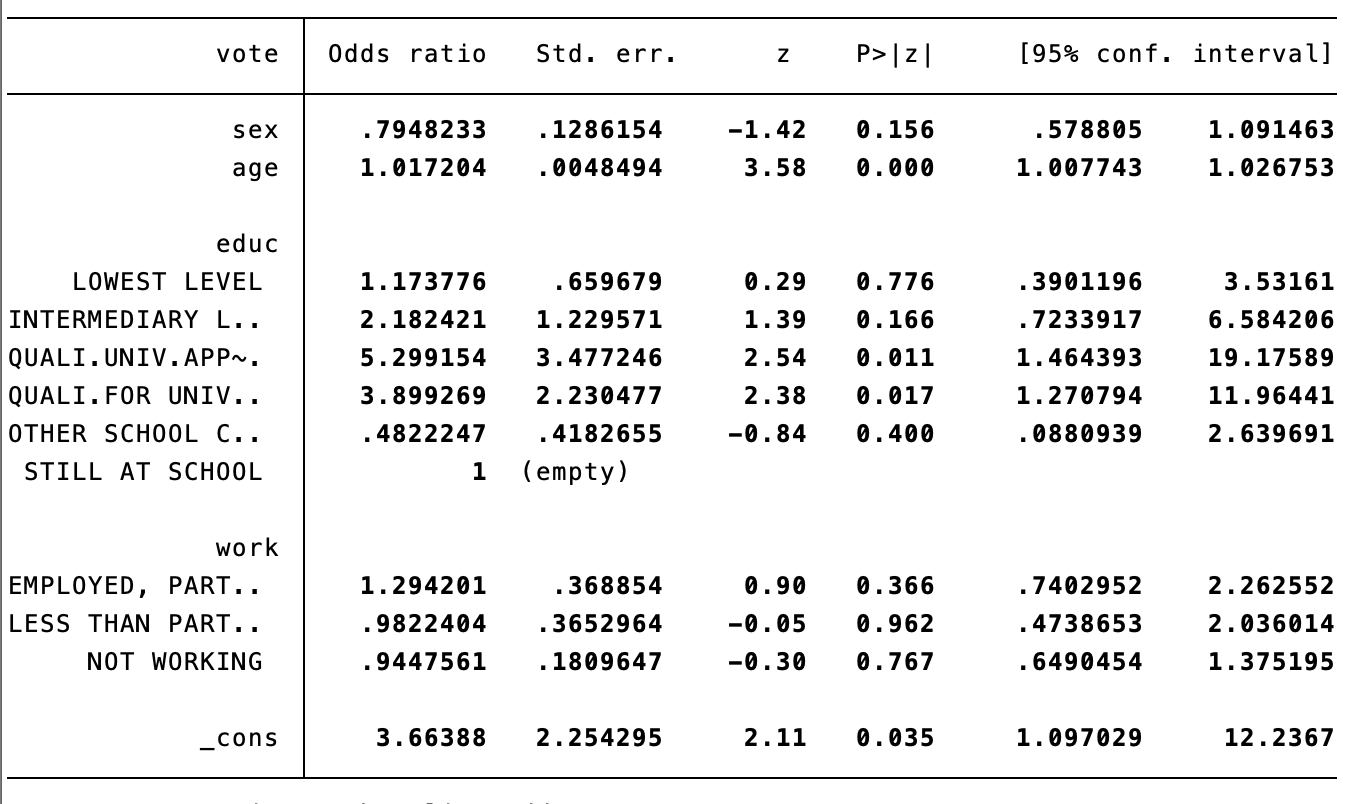
\includegraphics[width=13cm]{figs/11_log.png}
                \caption{Naïve Logit Regression}
                \label{fig_11_log}
            \end{figure}
            \begin{figure}[!htb]
                \centering 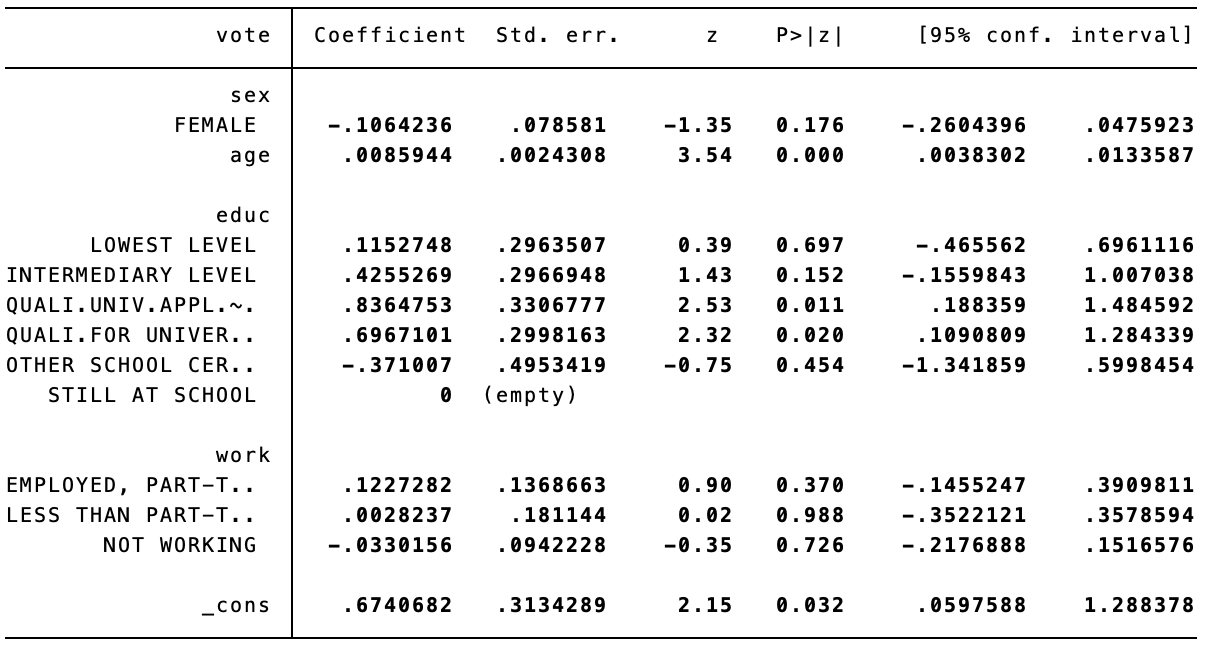
\includegraphics[width=13cm]{figs/11_prob.png}
                \caption{Naïve Probit Regression}
                \label{fig_11_prob}
            \end{figure}
            The estimates reported are the odds ratio. This simply states how likely a individual with a given characteristic is to vote (in this case) compared to the baseline characteristic. In the case of \texttt{sex}, male is base category so being female is associated being .79  as likely to vote, i.e. less likely than males.
                \newline\indent
            For continuous predictors the odds ratio simply imply that raising age by one year, on average is associated with 1.01 increase in probability to vote.
                \newline\indent
            Generally, having higher education makes an individual more likely to vote (compared to not having education). Being in part-time employment raises probability to vote, while less than part-time and being unemployment does not.
                \newline\indent
            The coefficients for the probit estimates of \eqref{eq_bin_probit} in Figure \ref{fig_11_prob} are not directly interpretable. The sign is interpretable however such that characteristics associated with positive effects (relative to their reference category) on probability to vote is
            \begin{itemize}
                \item 
                age, part-time employment (relative to full-time employment), less than part-time employment (relative to full-time employment). Low education level, middle education, university education (relative to no education)
            \end{itemize}
            those associated with negative effects are
            \begin{itemize}
                \item 
                female (relative to being male), other school certificatte (relative to no education), and not working (relative to full-time employment
            \end{itemize}
            
    
    \subsection{Marginal Effect at the Mean}
        The marginal effects at the mean of the logit model is presented in Figure \ref{fig_12_log_means} while effects for the probit model are in Figure \ref{fig_12_prob_means}.
            \begin{figure}[!htb]
                \centering
                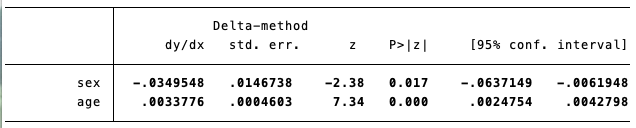
\includegraphics[width=10cm]{figs/12_log_means.png}
                \caption{Marginal Effects of Logit at the Mean}
                \label{fig_12_log_means}
            \end{figure}
            \begin{figure}[!htb]
                \centering
                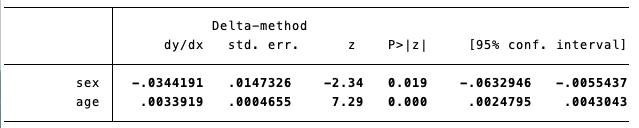
\includegraphics[width=10cm]{figs/12_prob_means.png}
                \caption{Marginal Effects of Probit at the Mean}
                \label{fig_12_prob_means}
            \end{figure}
        To find the probability of voting for a 26-year-old working male with an intermediate level of education, we simply substitute the coefficients from Figures \ref{fig_a1_log_coefs} and \ref{fig_11_prob} to the regression function as such
            \begin{align*}
                \frac{p}{1-p} &= \exp{(0.017*26 + 0.78*3)} \tag{Logit} 
                \\
                &= \exp{(2.78)}
                \\
                \Leftrightarrow \quad  \underline{\underline{p &= 0.941}}
            \end{align*}
            \begin{align*}
                p &= 1-\phi(-[0.0086*26 + 0.43*3])
                \tag{Probit}
                \\
                &= 1-\phi(-1.51)
                \\
                &= 1- 0.0655
                \\
                \Leftrightarrow \quad \underline{\underline{p &= 0.935}}
            \end{align*}
    
    \begin{samepage}
        \subsection{Binary Estimation}\label{subsec_bin_man_est}
            This code snippet below is developed in cooperation with Manohar Gannavarapu and John Searight as allowed by Prof. Wang.
                \begin{verbatim}
drop if pv01 < 0
gen vote2 = (pv01!=91)

global regressors "i.sex age i.educ i.work"

program define my_sigmoid
    args Y Xb
    qui replace `Y' = -ln(1+exp(-`Xb')) if $ML_y1==1
    qui replace `Y' = -`Xb' - ln(1+exp(-`Xb')) if $ML_y1==0
end

ml model lf my_sigmoid (vote2 = $regressors)
ml maximize
                 \end{verbatim}
            which outputs numerically equivalent estimations as Figure \ref{fig_a1_log_coefs} (same as Figure \ref{fig_11_log} but with coefficients instead of odds ratios).
        \end{samepage}